\documentclass{standalone}

\usepackage{tikz}
\usetikzlibrary{arrows}
\usetikzlibrary{decorations.markings}
\usetikzlibrary{calc}
\usetikzlibrary{shapes}

\begin{document}

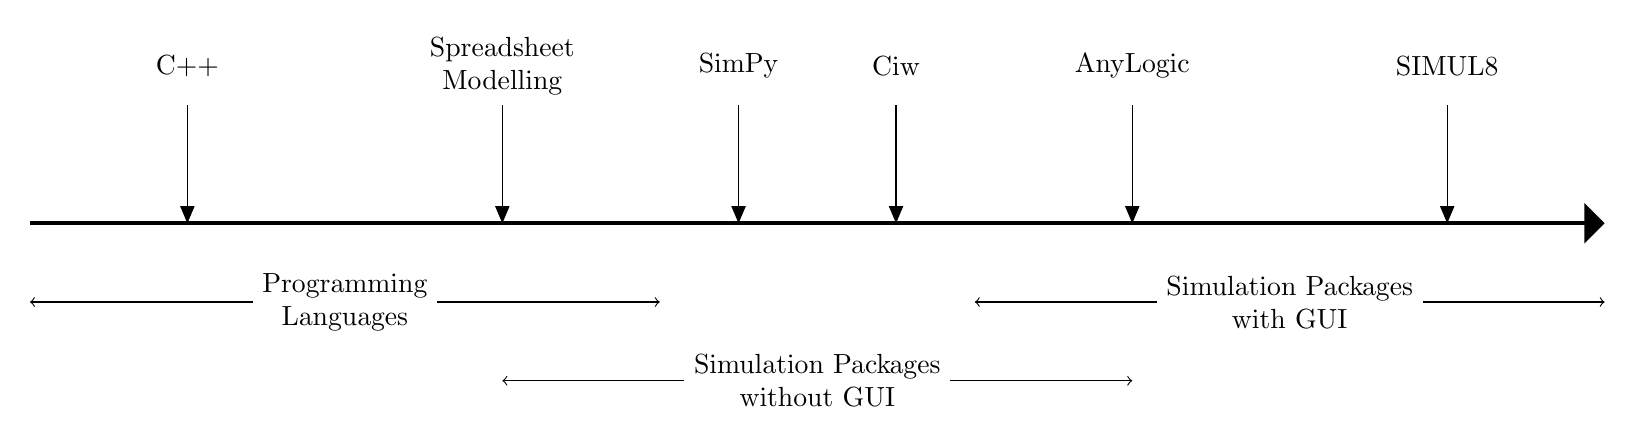
\begin{tikzpicture}

\draw[ultra thick, -triangle 90] (0, 0) -- (20, 0);

\node[align=center] (pl) at (4, -1) {Programming\\Languages};
\node[align=center] (nogui) at (10, -2) {Simulation Packages\\without GUI};
\node[align=center] (gui) at (16, -1) {Simulation Packages\\with GUI};

\draw[->] (pl) -- (0, -1);
\draw[->] (pl) -- (8, -1);

\draw[->] (nogui) -- (6, -2);
\draw[->] (nogui) -- (14, -2);

\draw[->] (gui) -- (12, -1);
\draw[->] (gui) -- (20, -1);

\draw[-triangle 45] (2, 1.5) -- (2, 0);
\draw[-triangle 45] (6, 1.5) -- (6, 0);
\draw[-triangle 45] (9, 1.5) -- (9, 0);
\draw[-triangle 45] (11, 1.5) -- (11, 0);
\draw[-triangle 45] (14, 1.5) -- (14, 0);
\draw[-triangle 45] (18, 1.5) -- (18, 0);

\node[align=center] at (2, 2) {C++};
\node[align=center] at (6, 2) {Spreadsheet\\Modelling};
\node[align=center] at (9, 2) {SimPy};
\node[align=center] at (11, 2) {Ciw};
\node[align=center] at (14, 2) {AnyLogic};
\node[align=center] at (18, 2) {SIMUL8};

\end{tikzpicture}

\end{document}
